% Lecture Template for ME3001-001-Tristan Hill - Spring 2017 - Fall 2017
% 
% Mechanical Engineering Analysis with MATLAB
%
% Introduction to Analysis

% Document settings
\documentclass[11pt]{article}
\usepackage[margin=1in]{geometry}
\usepackage[pdftex]{graphicx}
\usepackage{multirow}
\usepackage{setspace}
\usepackage{hyperref}
\usepackage{color,soul}
\usepackage{fancyvrb}
\usepackage{framed}
\usepackage{wasysym}
\usepackage{multicol}
\usepackage{ amssymb }
\usepackage{ bm }


\pagestyle{plain}
\setlength\parindent{0pt}
\hypersetup{
    bookmarks=true,         % show bookmarks bar?
    unicode=false,          % non-Latin characters in Acrobat’s bookmarks
    pdftoolbar=true,        % show Acrobat’s toolbar?
    pdfmenubar=true,        % show Acrobat’s menu?
    pdffitwindow=false,     % window fit to page when opened
    pdfstartview={FitH},    % fits the width of the page to the window
    pdftitle={My title},    % title
    pdfauthor={Author},     % author
    pdfsubject={Subject},   % subject of the document
    pdfcreator={Creator},   % creator of the document
    pdfproducer={Producer}, % producer of the document
    pdfkeywords={keyword1} {key2} {key3}, % list of keywords
    pdfnewwindow=true,      % links in new window
    colorlinks=true,       % false: boxed links; true: colored links
    linkcolor=red,          % color of internal links (change box color with linkbordercolor)
    citecolor=green,        % color of links to bibliography
    filecolor=magenta,      % color of file links
    urlcolor=blue           % color of external links
}

% assignment number 
\newcommand{\NUM}{1 } 
\newcommand{\VSpaceSize}{2mm} 
\newcommand{\HSpaceSize}{2mm} 

\newcommand{\Lagr}{\mathcal{L}}

\definecolor{mygray}{rgb}{.6, .6, .6}

\setulcolor{red} 
\setstcolor{green} 
\sethlcolor{mygray} 

\begin{document}

\textbf{ \LARGE ME 3050 Lecture - State Space Models} \vspace{3mm}\\
\textbf{ \hspace*{5mm}Tristan W. Hill - Tennessee Technological University - Spring 2020 } \vspace{3mm}\\

\Large
\begin{itemize}

\item \textbf{ \Large We have been studying very simple models: } \\ \\

\scalebox{1.5}{$m\dot{v} +cv=f(t)$} \\ 

and \\

\scalebox{1.5}{$m\ddot{x} +c\dot{x} +kx=f(t)$} \\


\item \textbf{ \Large These accurately describe all mechanical systems ... right? }\vspace{2mm}\\

\item \textbf{ \Large No, but we can improve them by adding complexity. How?  }\vspace{5mm}\\
\Large

	Improvements/Additions to the model:\\
	\begin{itemize}
		\item  

		\item

		\item
	\end{itemize}
	

\newpage
\item \textbf{ \Large Higher Order Models} - Mechanical systems involve the interactions between multiple rigid bodys. This can be seen in many examples.
\Large

	\begin{itemize}
		\item  Automobile Suspension

		\item Beam Deflection (FEA)

		\item Tether Based Space Travel

		\item Virtually Everything!

	\end{itemize}

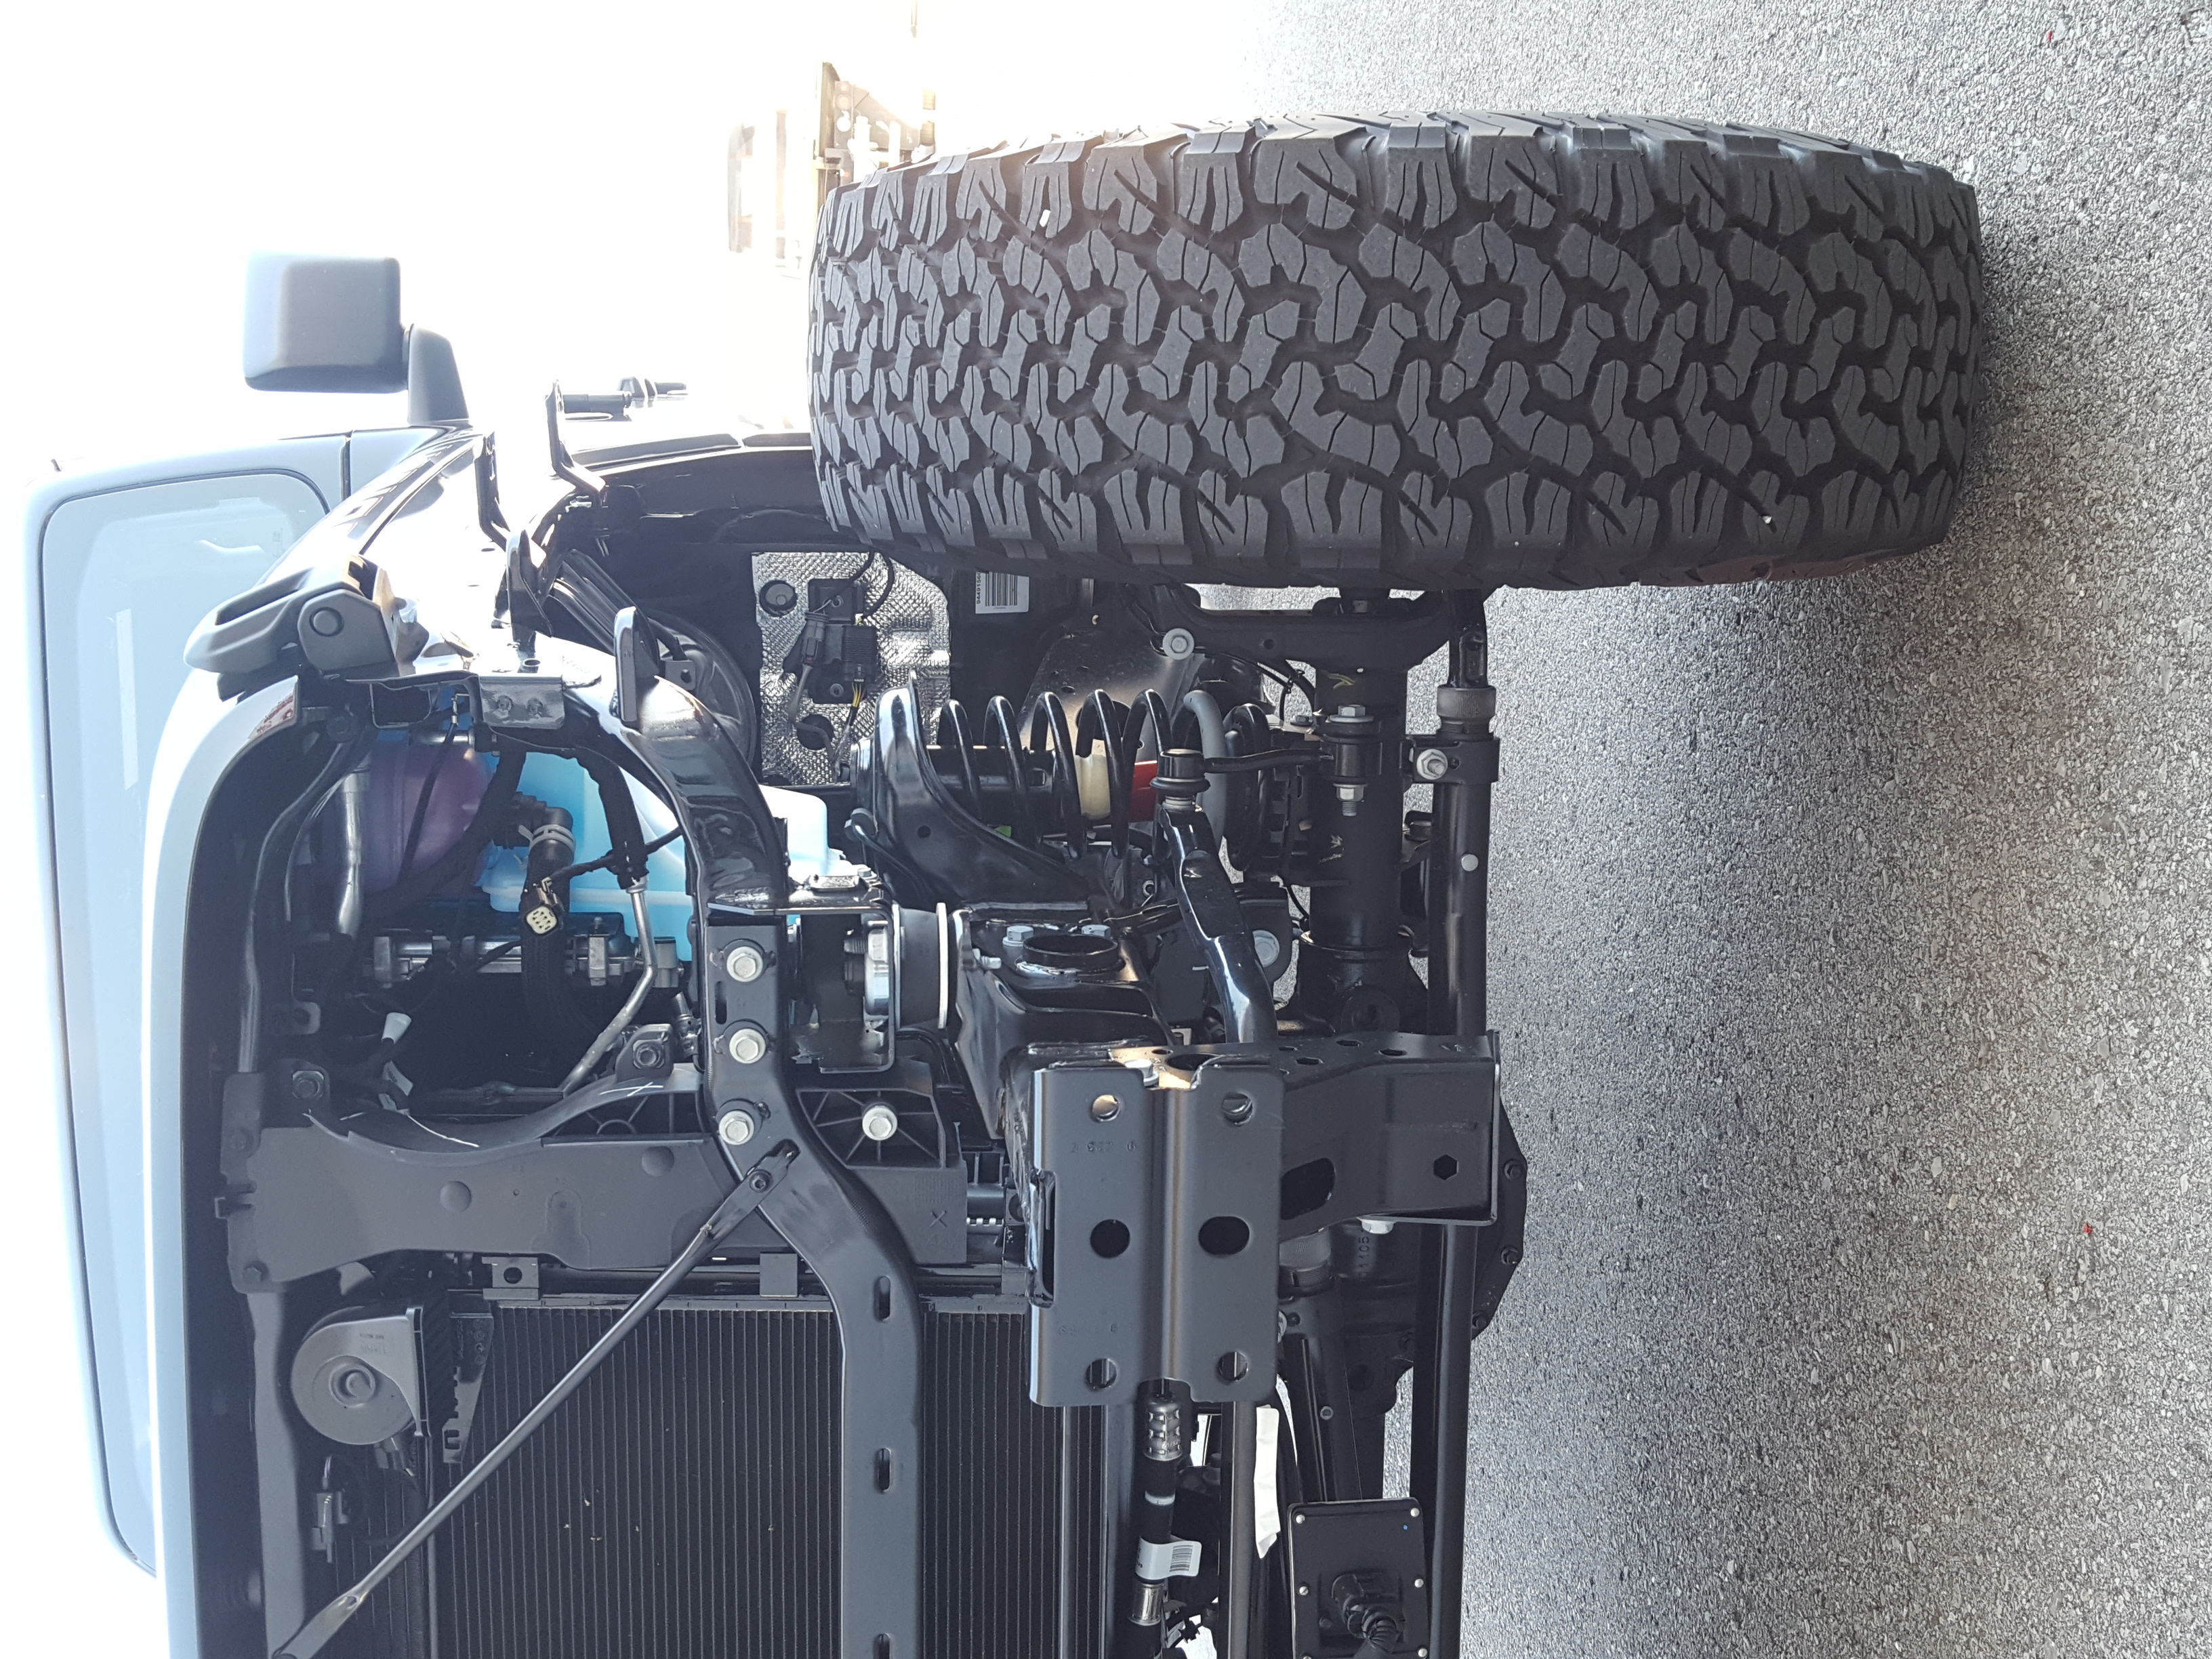
\includegraphics[scale=.05,angle=-90,origin=c]{jeep_01.jpg} \hspace{10mm}  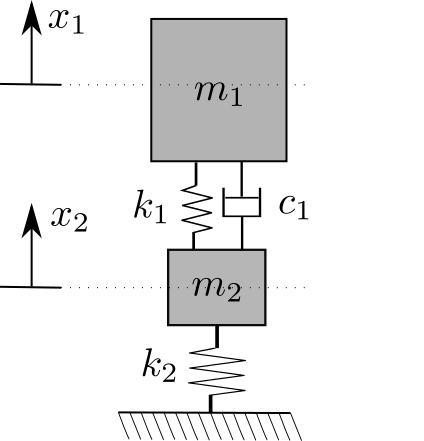
\includegraphics[scale=.5]{mass_spring_2dof.png}\\

\item \textbf{ \Large Higher Order EOMs} - There is one equation of motion for Each body. \\ In class we derived the following EOMs for the suspension model shown. \\
\Large

	
	Equation of Motion for Mass 1: \\

	\scalebox{1.25}{$m_1\ddot{x}_1+c_1(\dot{x}_1-\dot{x}_2)+k_1(x_1-x_2)=0$} \vspace{5mm}\\

	Equation of Motion for Mass 1: \\

	\scalebox{1.25}{$m_2\ddot{x}_2+k_2x_2-c_1(\dot{x}_1-\dot{x}_2)-k_1(x_1-x_2)=0$} \vspace{5mm}\\

	We want to find a solution to this system of differential equations. \\ Find $x_1(t)$ and $x_2(t)$ due to given initial condtions $x_{1o}, x_{2o}, v_{1o}$ , and $v_{2o}$.\\

\item \textbf{ \Large State Space Model Representation (textbook 5.2) } - 

	\begin{itemize}

		\item {\it commonly used} for system models \\

		\item useful for {\it numerical simulation}\\

		\item used in the area of {\it automatic control}\\

		\item an ODE system has an equivalent State Space Model representation\\

	\end{itemize}

\item \textbf{ \Large The State Equation} - Standard Form \\\\

	\scalebox{1.5}{$\bm{ \dot{x} } = \bm{Ax} + \bm{Bu}$} \vspace{0mm}\\

	\begin{itemize}

		\item there are n {\it state variables} or {\it states} called $x_1 - x_n$ 
		\item there are m {\it inputs} called $u_1 - u_m$ 
		\item the {\it state vector} $\bm{x}$ is a collumn vector with {\it n} rows
		\item the {\it system matrix} $\bm{A}$ is a square matrix {\it n} rows and {\it n} columns.
		\item the {\it input vector} $\bm{u}$ is a column vector with {\it m} rows.
		\item the {\it control or input matrix} $\bm{B}$ is a matrix with {\it n} rows and {\it m} columns. \\

	\end{itemize}
\item \textbf{ \Large The Output Equation} - Standard Form \\\\

	\scalebox{1.5}{$\bm{y } = \bm{Cx} + \bm{Du}$} \vspace{0mm}\\

	\begin{itemize}


		\item the {\it output vector} $\bm{y}$ is a collumn vector with {\it p} rows
		\item the {\it output matrix} $\bm{C}$ is a square matrix {\it p} rows and {\it n} columns.
		\item the {\it control matrix} $\bm{D}$ is a matrix with {\it p} rows and {\it m} columns.

	\end{itemize}


\item \textbf{ \Large Example} - Let's do a simple example before we do the more complex suspension model. You can use this for any system\ of {\it linear} ODEs. \\\\

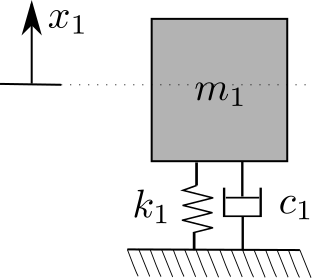
\includegraphics[scale=.5]{mass_spring_1dof.png} \\
\end{itemize}

\end{document}



